\newcommand{\equal}{=\space}
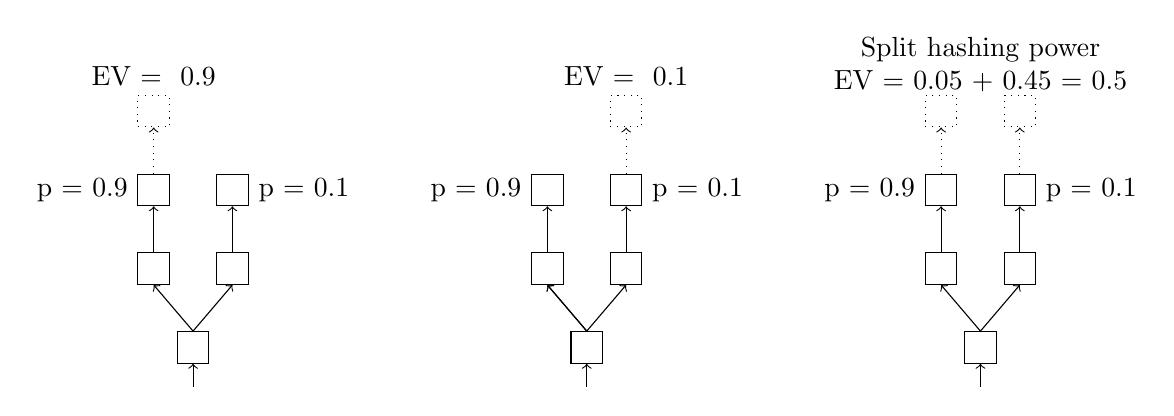
\begin{tikzpicture}
	[block/.style={rectangle,draw=black, inner sep=0pt,minimum size=4mm},
	appendingBlock/.style={rectangle,draw=black, inner sep=0pt,minimum size=4mm}]
	
	% first chain EV=0.1
	\node (a) at ( 0,0 ) [block] {};
	\node (b) at ( -0.5,1 ) [block] {};
	\node (c) at ( 0.5,1 ) [block] {};
	\node (d) at ( -0.5,2 ) [block, label=180:p \equal0.9] {};
	\node (e) at ( 0.5,2 ) [block, label=0:p \equal0.1] {};
	\node (f) at ( -0.5,3 ) [appendingBlock, dotted, label=90:EV \equal\space0.9] {};
	
	\draw[->] (0, -0.5) -- (a);
	\draw [->] (a.north) -- (b.south);    
	\draw [->] (a.north) -- (c.south);
	\draw [->] (b.north) -- (d.south);
	\draw [->] (c.north) -- (e.south);
	\draw [->, dotted] (d.north) -- (f.south);
	
	
	% second chain EV=0.1
	\node (g) at ( 5,0 ) [block] {};
	\node (h) at ( 4.5,1 ) [block] {};
	\node (i) at ( 5.5,1 ) [block] {};
	\node (j) at ( 4.5,2 ) [block, label=180:p \equal0.9] {};
	\node (k) at ( 5.5,2 ) [block, label=0:p \equal0.1] {};
	\node (l) at ( 5.5,3 ) [appendingBlock, dotted, label=90:EV \equal\space0.1] {};
	
	\draw[->] (5, -0.5) -- (g);
	\draw [->] (g.north) -- (h.south);    
	\draw [->] (g.north) -- (h.south);    
	\draw [->] (g.north) -- (i.south);
	\draw [->] (h.north) -- (j.south);
	\draw [->] (i.north) -- (k.south);
	\draw [->, dotted] (k.north) -- (l.south);
	
	% third chain EV=1
	\node (m) at ( 10,0 ) [block] {};
	\node (n) at ( 9.5,1 ) [block] {};
	\node (o) at ( 10.5,1 ) [block] {};
	\node (p) at ( 9.5,2 ) [block, label=180:p \equal0.9] {};
	\node (q) at ( 10.5,2 ) [block, label=0:p \equal0.1] {};
	\node (r) at ( 9.5,3 ) [appendingBlock, dotted] {};
	\node (s) at ( 10.5,3 ) [appendingBlock, dotted] {};
	\node (t) at ( 10,3 ) [label={[align=center]Split hashing power\\EV \equal0.05 + 0.45 \equal0.5}] {};
	
	\draw[->] (10, -0.5) -- (m);
	\draw [->] (m.north) -- (n.south);    
	\draw [->] (m.north) -- (o.south);
	\draw [->] (n.north) -- (p.south);
	\draw [->] (o.north) -- (q.south);
	\draw [->, dotted] (p.north) -- (r.south);
	\draw [->, dotted] (q.north) -- (s.south);

\end{tikzpicture}
